\chapter{PLANTEAMIENTO DEL PROBLEMA}
\section{Descripción de la Realidad Problemática}

La situación de atención médica en las áreas rurales de Perú es una realidad compleja y desafiante. Imagine comunidades enclavadas en paisajes montañosos y remotos, donde acceder a servicios médicos básicos es una odisea. La falta de infraestructura adecuada y la escasez de profesionales de la salud crean una brecha significativa en el acceso a la atención médica, dejando a muchas personas sin la ayuda que necesitan cuando más la necesitan. Según el Instituto Nacional de Estadística e Informática (INEI), en 2022, solo el 20\% pertenece a la población rural, en comparación con el 80\% de la población urbana. Esto significa que millones de peruanos en áreas rurales son más vulnerables a enfermedades y muertes evitables.

\begin{figure}[h]
	\begin{center}
		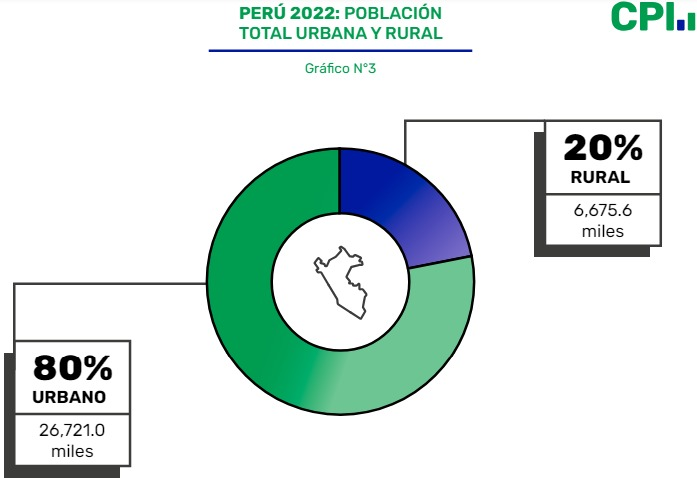
\includegraphics[width=0.6\textwidth]{1/figures/INEITOTAL.jpeg}
		\caption{Total de poblacion rural y urbana. Fuente: \cite{gl_inei}}
		\label{1:fig}
	\end{center}
\end{figure}

Ademas, los datos oficiales respaldan estas realidades duras. Según el Ministerio de Salud de Perú, en el 2021, más del 70\% de la población rural carecía de acceso regular a servicios médicos adecuados. Esto no es solo una estadística fría, sino una narrativa de vidas afectadas, enfermedades no tratadas y vidas que podrían haberse salvado con una atención médica oportuna.

\begin{figure}[h]
	\begin{center}
		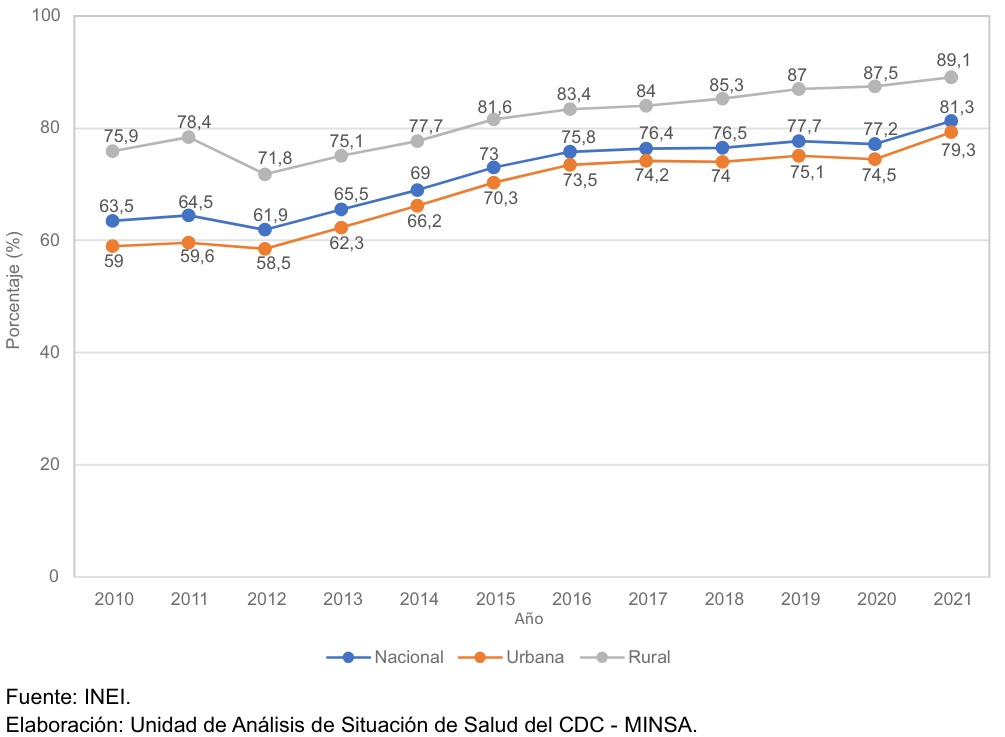
\includegraphics[width=0.6\textwidth]{1/figures/MINSA.jpeg}
		\caption{Porcentaje de acceso a atencion medica. Fuente: \cite{gl_inei}}
		\label{2:fig}
	\end{center}
\end{figure}

Durante el período comprendido entre 2022 y 2024, la pandemia de COVID-19 solo ha intensificado estos desafíos. Los recursos y la atención se desplazaron hacia la respuesta a la pandemia, dejando otras necesidades de salud pública en segundo plano. Las comunidades rurales se encontraron aún más marginadas, enfrentando una atención médica aún más limitada y fragmentada.

Sin embargo, entre estas sombras de dificultades, hay un rayo de esperanza en la forma de la tecnología. El aumento del acceso a teléfonos móviles en áreas rurales ofrece una oportunidad única para brindar servicios médicos básicos a través de plataformas digitales, incluso en las zonas más remotas del país. Es aquí donde entra en juego la idea de un chatbot médico.

Imagínese un sistema donde las personas en las comunidades rurales pueden acceder a información médica básica, hacer consultas sobre síntomas y recibir orientación sobre cómo buscar atención médica, todo desde la comodidad de sus teléfonos móviles. Esto no solo podría salvar vidas, sino también aliviar la carga sobre los pocos centros de salud disponibles en estas áreas.

Pero, por supuesto, hay obstáculos por superar. La adaptación cultural, la capacitación de los usuarios y la garantía de la precisión de la información son solo algunos de los desafíos que enfrenta esta iniciativa. Además, la conectividad limitada en algunas áreas rurales plantea desafíos adicionales para garantizar un acceso efectivo a la aplicación.

La implementación de Chatbots Médicos en áreas rurales del Perú tiene el potencial de mejorar significativamente el acceso a la atención médica para millones de personas. Estos sistemas pueden proporcionar información y asesoramiento médico de manera remota, sin necesidad de que un médico esté presente físicamente. Además, los Chatbots Médicos pueden ayudar a los pacientes a programar citas, recordarles que tomen sus medicamentos y monitorear su progreso. 


%\begin{figure}[h]
%	\begin{center}
%		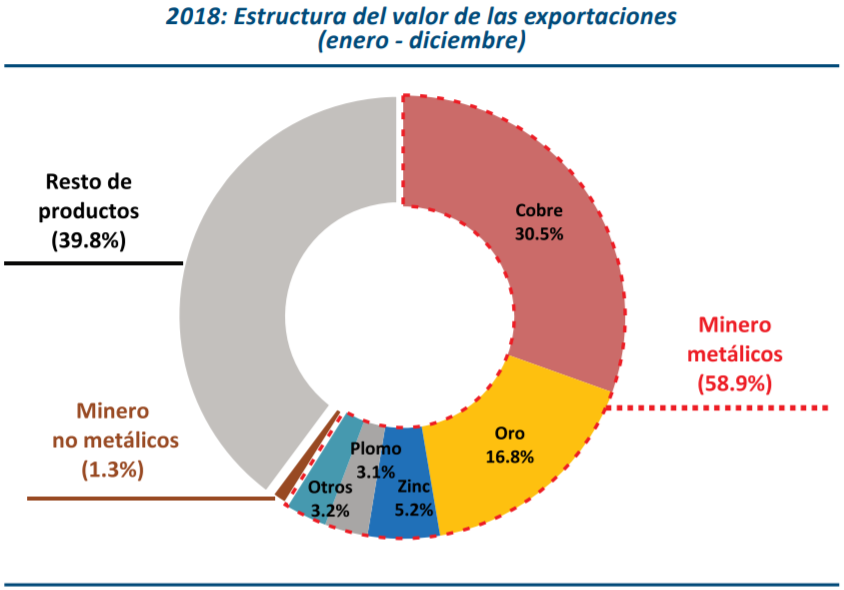
\includegraphics[width=0.8\textwidth]{1/figures/estructura_exportaciones_peru.png}
%		\caption{Estructura del valor de las exportaciones peruanas en el año 2018. Fuente: \cite{cu_ministerioPeru_statsminas}}
%		\label{1:fig2}
%	\end{center}
%\end{figure}

%\begin{figure}[h]
%	\begin{center}
%		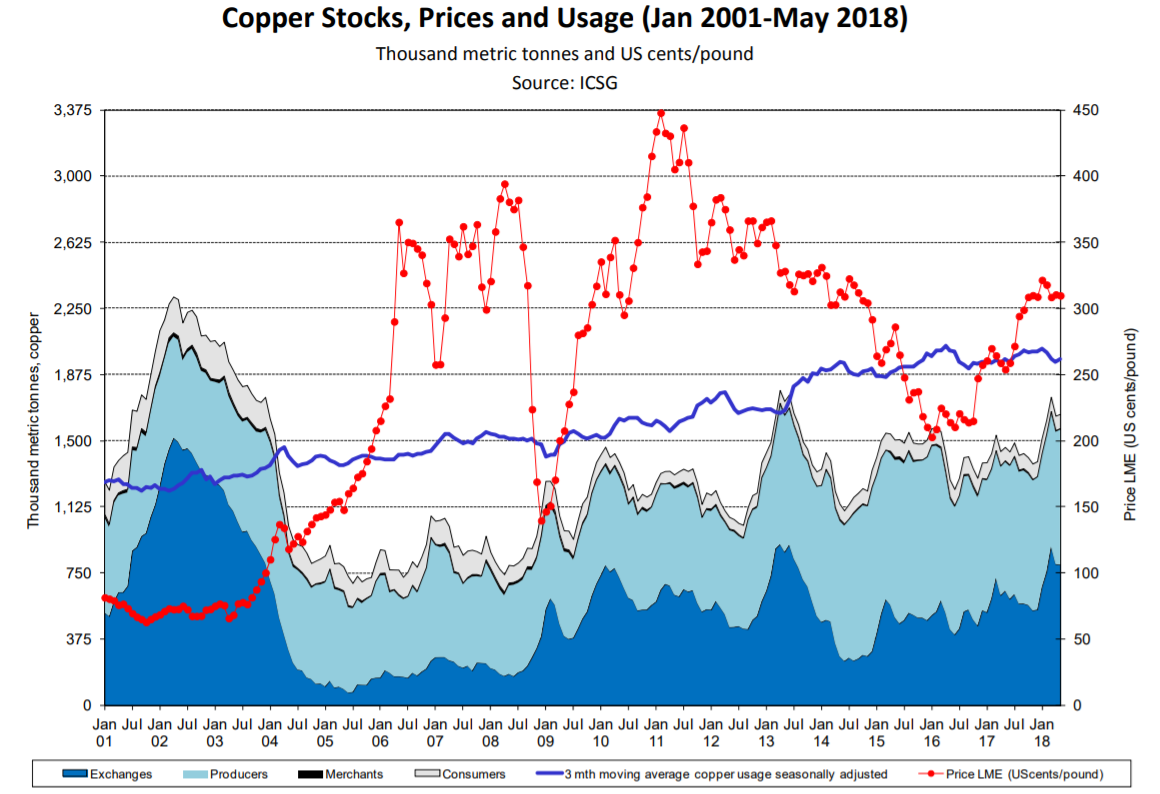
\includegraphics[width=0.8\textwidth]{1/figures/copper_stocks_prices_usage.png}
%		\caption{Precio, stocks y uso del cobre (cantidad en miles de toneladas y precio en centavos por libra). Fuente: \cite{cu_internationalcopper2018}}	
%		\label{1:fig3}
%	\end{center}
%\end{figure}

\section{Formulación del Problema}

%Para lefecto \parencite{ot_marti2018manual}. 


%Una vez elaborado el diagrama (véase Anexo 1), 

\subsection{Problema General}
\newcommand{\ProblemaGeneral}{
¿De qué manera la implementación de un chatbot médico puede mejorar el acceso a servicios de salud en las zonas rurales de Perú?
}
\ProblemaGeneral
\subsection{Problemas Espec\'{i}ficos}
\newcommand{\Pbone}{
¿Cuáles son los desafíos y las oportunidades para la implementación de chatbots médicos en áreas rurales?
}
\newcommand{\Pbtwo}{
¿Qué características y funcionalidades debe tener un chatbot médico para ser efectivo en áreas rurales?
}
\newcommand{\Pbthree}{
¿Qué estrategias se pueden utilizar para promover la adopción y el uso del chatbot médico entre las poblaciones rurales?
}
\newcommand{\Pbfour}{
¿Qué métricas se pueden utilizar para evaluar la efectividad del chatbot médico en la mejora del acceso a la atención médica y los resultados de salud en las poblaciones rurales?
}


\begin{itemize}
	\item \Pbone
	\item \Pbtwo
	\item \Pbthree
	\item \Pbfour

\end{itemize}

\section{Objetivos de la Investigación}

%Para la formulación de los objetivos de la presente investigación se elaboró un «árbol de objetivos» (véase Anexo 2) 
\subsection{Objetivo General}
\newcommand{\ObjetivoGeneral}{
Implementar un chatbot médico efectivo y sostenible para brindar servicios de salud de calidad a las poblaciones rurales en Perú
}
\ObjetivoGeneral
\subsection{Objetivos Espec\'{i}ficos}
\newcommand{\Objone}{
Diseñar un chatbot médico capaz de brindar asesoramiento y orientación médica confiable, actuando como un complemento a los profesionales de la salud en áreas con escasez de personal médico.
}
\newcommand{\Objtwo}{
Implementar el chatbot médico en áreas rurales utilizando tecnologías accesibles y asequibles, como dispositivos móviles y conectividad a internet local.
}
\newcommand{\Objthree}{
Garantizar la confiabilidad y la precisión de la información proporcionada por el chatbot médico a través de mecanismos de revisión y actualización constantes.
}
\newcommand{\Objfour}{
Evaluar la confiabilidad, precisión y efectividad del chatbot médico en un estudio piloto.
}


\begin{itemize}
	\item {\Objone}
	\item {\Objtwo}
	\item {\Objthree}
	\item {\Objfour}

\end{itemize}

\section{Justificación de la Investigación}

\subsection{Teórica}
Esta investigación se realiza 

\subsection{Práctica}
Al culminar la investigación 

\subsection{Metodológica}. 

\section{Delimitación del Estudio}

\subsection{Espacial}
Para la presente investigación 

\subsection{Temporal}
Los datos que serán necesari. 

\subsection{Conceptual}
Esta investigación se 

\section{Hipótesis}

\subsection{Hipótesis General}
\newcommand{\HipotesisGeneral}{
La implementación de un chatbot médico puede mejorar significativamente el acceso a servicios médicos de calidad para las poblaciones rurales.
}
\HipotesisGeneral
\subsection{Hipótesis Específicas}
\newcommand{\Hone}{
La implementación de un chatbot médico en áreas rurales de Perú aumentará la tasa de consultas médicas atendidas a distancia, disminuyendo la necesidad de desplazamientos largos y costosos para recibir atención presencial.
}
\newcommand{\Htwo}{
El uso del chatbot médico reducirá el tiempo promedio de espera para recibir atención médica en áreas rurales de Perú, agilizando el proceso de diagnóstico y tratamiento de enfermedades.
}
\newcommand{\Hthree}{
El chatbot médico mejorará la satisfacción de los usuarios con la atención médica recibida en áreas rurales de Perú, al brindarles un servicio accesible, personalizado y oportuno.
}
\newcommand{\Hfour}{
La implementación del chatbot médico contribuirá a la reducción de las disparidades en salud entre las poblaciones rurales y urbanas en Perú, democratizando el acceso a información y servicios médicos de calidad.
}
\begin{itemize}
	\item \Hone
	\item \Htwo
	\item \Hthree
	\item \Hfour

\end{itemize}

\subsection{Matriz de Consistencia}
A continuación se presenta la matriz de consistencia elaborada para la presente investigación (véase Anexo \ref{1:table}).

